\PassOptionsToPackage{unicode=true}{hyperref} % options for packages loaded elsewhere
\PassOptionsToPackage{hyphens}{url}
%
\documentclass[14pt,ignorenonframetext,]{beamer}
\usepackage{pgfpages}
\setbeamertemplate{caption}[numbered]
\setbeamertemplate{caption label separator}{: }
\setbeamercolor{caption name}{fg=normal text.fg}
\beamertemplatenavigationsymbolsempty
% Prevent slide breaks in the middle of a paragraph:
\widowpenalties 1 10000
\raggedbottom
\setbeamertemplate{part page}{
\centering
\begin{beamercolorbox}[sep=16pt,center]{part title}
  \usebeamerfont{part title}\insertpart\par
\end{beamercolorbox}
}
\setbeamertemplate{section page}{
\centering
\begin{beamercolorbox}[sep=12pt,center]{part title}
  \usebeamerfont{section title}\insertsection\par
\end{beamercolorbox}
}
\setbeamertemplate{subsection page}{
\centering
\begin{beamercolorbox}[sep=8pt,center]{part title}
  \usebeamerfont{subsection title}\insertsubsection\par
\end{beamercolorbox}
}
\AtBeginPart{
  \frame{\partpage}
}
\AtBeginSection{
  \ifbibliography
  \else
    \frame{\sectionpage}
  \fi
}
\AtBeginSubsection{
  \frame{\subsectionpage}
}
\usepackage{lmodern}
\usepackage{amssymb,amsmath}
\usepackage{ifxetex,ifluatex}
\usepackage{fixltx2e} % provides \textsubscript
\ifnum 0\ifxetex 1\fi\ifluatex 1\fi=0 % if pdftex
  \usepackage[T1]{fontenc}
  \usepackage[utf8]{inputenc}
  \usepackage{textcomp} % provides euro and other symbols
\else % if luatex or xelatex
  \usepackage{unicode-math}
  \defaultfontfeatures{Ligatures=TeX,Scale=MatchLowercase}
\fi
\usetheme[]{metropolis}
% use upquote if available, for straight quotes in verbatim environments
\IfFileExists{upquote.sty}{\usepackage{upquote}}{}
% use microtype if available
\IfFileExists{microtype.sty}{%
\usepackage[]{microtype}
\UseMicrotypeSet[protrusion]{basicmath} % disable protrusion for tt fonts
}{}
\IfFileExists{parskip.sty}{%
\usepackage{parskip}
}{% else
\setlength{\parindent}{0pt}
\setlength{\parskip}{6pt plus 2pt minus 1pt}
}
\usepackage{hyperref}
\hypersetup{
            pdftitle={Well Modeling and Batch Automation},
            pdfauthor={Alfonso R. Reyes},
            pdfborder={0 0 0},
            breaklinks=true}
\urlstyle{same}  % don't use monospace font for urls
\newif\ifbibliography
\setlength{\emergencystretch}{3em}  % prevent overfull lines
\providecommand{\tightlist}{%
  \setlength{\itemsep}{0pt}\setlength{\parskip}{0pt}}
\setcounter{secnumdepth}{0}

% set default figure placement to htbp
\makeatletter
\def\fps@figure{htbp}
\makeatother

% \usetheme{metropolis}
% \usepackage{../metropolis/beamerthememetropolis}
\usepackage{../metropolis/beamerthememetropolis}

\usepackage{appendixnumberbeamer}

\usepackage{booktabs}
\usepackage[scale=2]{ccicons}

\usepackage{pgfplots}
\usepgfplotslibrary{dateplot}

\usepackage{xspace}
\newcommand{\themename}{\textbf{\textsc{metropolis}}\xspace}

\metroset{titleformat frame=smallcaps}

% Add section numbers in TOC
% https://tex.stackexchange.com/a/44998/173708
\setbeamertemplate{section in toc}[sections numbered]

%%% Local Variables:
%%% mode: latex
%%% TeX-master: t
%%% End:


% make background color for title of the slides green
% https://tex.stackexchange.com/a/360349/173708
\definecolor{OilGainsGreen}{RGB}{85, 130, 5}    % Fidelity green normal
\setbeamercolor{frametitle}{bg=OilGainsGreen}   % do not change foreground color

% set folder for figures
\graphicspath{{figs/}}


% remove the [rt] keyword. Offset and increase to maximum size
% https://tex.stackexchange.com/a/412707/173708
\titlegraphic{%
  \begin{picture}(0,0)
    \put(154.5,-107){\makebox(0,0){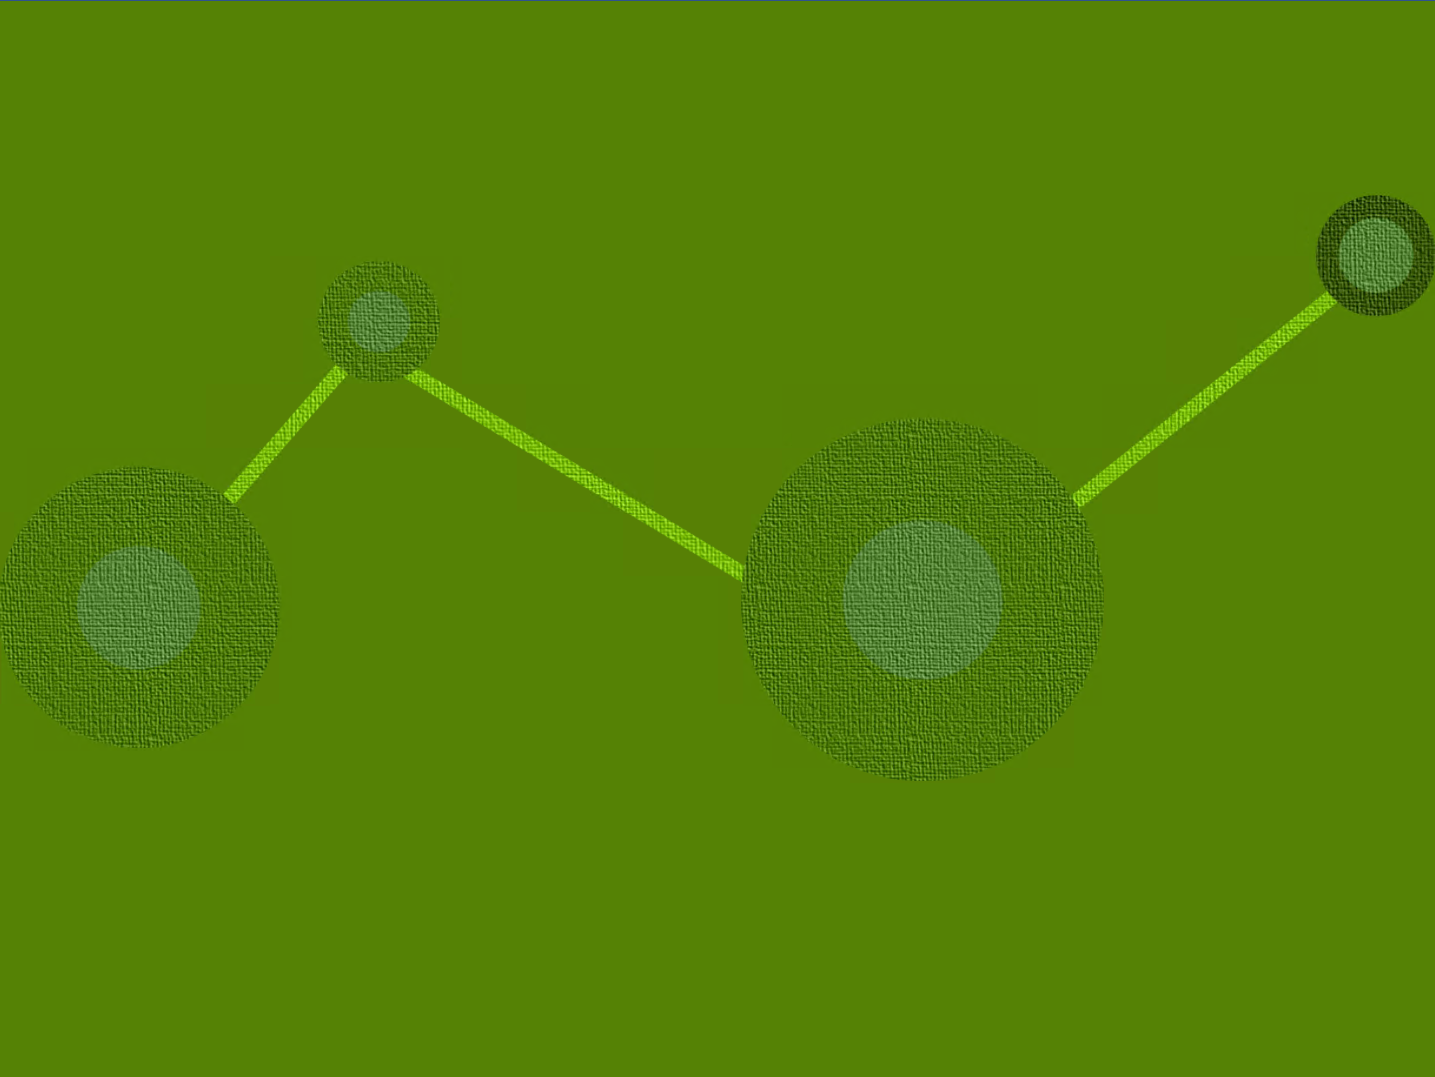
\includegraphics[width=\paperwidth,height=\paperheight]{OilGainsTitleSlide2}}}
  \end{picture}}


% change color of title and subtitle
\definecolor{OilGainsGreen}{RGB}{85, 130, 5}  % Fidelity green normal
\setbeamercolor{title}{fg=white,bg=OilGainsGreen}
\setbeamercolor{subtitle}{fg=yellow,bg=OilGainsGreen}
\setbeamercolor{author}{fg=white,bg=OilGainsGreen}
\setbeamercolor{date}{fg=white,bg=OilGainsGreen}
\setbeamercolor{institute}{fg=yellow,bg=OilGainsGreen}

% change color of the progress bar and title separator
\definecolor{blueucl}{RGB}{0,87,156} %which is the color of my university
\setbeamercolor{progress bar}{fg=blueucl}
\setbeamercolor{title separator}{fg=lightgray} % color of the title separator
\setbeamercolor{progress bar in head/foot}{fg=blueucl}
\setbeamercolor{progress bar in section page}{fg=OilGainsGreen}


% change color standout slide
% https://github.com/matze/mtheme/issues/234
\definecolor{myGreen}{RGB}{30,98,56}
\definecolor{myGold}{RGB}{226,168,43}
% keep colors white and OilGainsGreen
\setbeamercolor{palette primary}{fg=white, bg=OilGainsGreen}

% change TOC color
% https://tex.stackexchange.com/a/29332/173708
\colorlet{mycolor}{orange!80!black}% change this color to suit your needs
\setbeamercolor{section in toc}{fg=mycolor}
\setbeamercolor{subsection in toc shaded}{fg=black}

% change thickness of progress bar and title separator
% https://github.com/matze/mtheme/issues/237
\makeatletter
\setlength{\metropolis@titleseparator@linewidth}{0.25pt}
\setlength{\metropolis@progressonsectionpage@linewidth}{2pt}
\setlength{\metropolis@progressinheadfoot@linewidth}{2pt}
\makeatother

% \logo{the logo \raisebox{0.5cm}{
\includegraphics[width=1cm]{logo}}\hspace*{\textwidth}}

% place the logo at the bottom of each slide
% https://tex.stackexchange.com/a/341702/173708
\usepackage{graphbox}
\setbeamertemplate{footline}{%
    
\includegraphics[align=c, height=0.45cm]{oilgains-alegr}%
    \hfill%
    \usebeamercolor[fg]{page number in head/foot}%
    \usebeamerfont{page number in head/foot}%
    \insertframenumber\,/\,\inserttotalframenumber\kern1em%
}

% Plenty of room
\setbeamersize{text margin left=2em,text margin right=2em}

% Figure placement using textpos
\usepackage{graphicx}
\usepackage[absolute,overlay]{textpos}
\setlength{\TPHorizModule}{1cm}
\setlength{\TPVertModule}{1cm}
\def\placefig#1#2#3#4{\begin{textblock}{.1}(#1,#2)\rlap{\includegraphics[#3]{#4}}\end{textblock}}


% define maxwidth and maxheight
\def\maxwidth{11.5cm}
\def\maxheight{8cm}
% Scale images if necessary, so that they will not overflow the page
% margins by default, and it is still possible to overwrite the defaults
% using explicit options in \includegraphics[width, height, ...]{}
\setkeys{Gin}{width=\maxwidth,height=\maxheight,keepaspectratio}

% define fullwidth and fullheight
% \def\fullwidth#1{\vspace*{0.225cm}\par\centerline{\includegraphics[width=20cm]{#1}}}
% \def\fullheight#1{\vspace*{0.0cm}\par\centerline{\includegraphics[height=12cm]{#1}}}
\def\fullwidth#1{\vspace*{-0.2cm}\par\centerline{\includegraphics[width=20cm]{#1}}}
\def\fullheight#1{\vspace*{-0.2cm}\par\centerline{\includegraphics[height=12cm]{#1}}}

\title{Well Modeling and Batch Automation}
\author{Alfonso R. Reyes}
\date{April 2019}

\begin{document}
\frame{\titlepage}

\hypertarget{well-modeling-and-batch-automation}{%
\section{Well modeling and batch
automation}\label{well-modeling-and-batch-automation}}

\begin{frame}{Why automating well modeling?}
\protect\hypertarget{why-automating-well-modeling}{}

\fontsize{13}{15}\sf

\begin{itemize}
\tightlist
\item
  Modeling takes a long time
\item
  It is laborious to calibrate and modify each model
\item
  It is easy for ten wells
\item
  But very hard on 25, 50, 100, 200+ wells
\item
  And when you finish the first batch of well tests \ldots{}
\item
  \ldots{} it comes another \ldots{}
\item
  One production optimization cycle could take months
\end{itemize}

\end{frame}

\begin{frame}{How is it like now?}
\protect\hypertarget{how-is-it-like-now}{}

\fontsize{13}{15}\sf

\begin{itemize}
\tightlist
\item
  Models take from 3-9 months to build \[f(N)\] where \(N\) is the
  number of wells
\item
  Models do not immediately match
\item
  Wrong models left as-is to move on to network optimization
\item
  Get wrong results from the optimization solver
\item
  In the end: \newline \fontsize{12}{14}\sf
  \alert{Production Optimization is great but becomes unreliable}
\end{itemize}

\end{frame}

\begin{frame}{Sample multiwell table}
\protect\hypertarget{sample-multiwell-table}{}

\fullwidth{well_scanner_output_2}

\end{frame}

\hypertarget{statistical-analysis}{%
\section{Statistical analysis}\label{statistical-analysis}}

\begin{frame}{Statistical analysis}
\protect\hypertarget{statistical-analysis-1}{}

\begin{alertblock}{}
Statistical Analysis makes a difference
\end{alertblock}

\vspace{1.0cm}

\fontsize{13}{15}\sf

\begin{itemize}
\tightlist
\item
  All wells data get into a tabular format: dataframe
\item
  Every well is a row (observation)
\item
  Well parameters become columns or variables
\item
  Tables make easier to spot problems with the data
\item
  Well scanning can be done on a directory or drive
\item
  Well variables (columns) are selectable
\end{itemize}

\end{frame}

\begin{frame}{Advantages}
\protect\hypertarget{advantages}{}

\begin{itemize}
\tightlist
\item
  Matching the models gets certain
\item
  Reliable Well Models Construction
\item
  Issues with well tests get more manageable
\item
  Learn to trust the data
\end{itemize}

\end{frame}

\hypertarget{batch-automation}{%
\section{Batch Automation}\label{batch-automation}}

\begin{frame}{Current wokflow of model building}
\protect\hypertarget{current-wokflow-of-model-building}{}

\fontsize{13}{15}\sf
\begin{alertblock}{}
  Why doesn't work most of the time
\end{alertblock}

\vspace{1.0cm}

\begin{itemize}
\tightlist
\item
  You deal with one well at a time
\item
  Cannot see the variation between wells: isolated
\item
  Well data cannot be compared
\item
  There is no data structure in place
\item
  No input validation but by the software
\item
  Model files are in binary format
\end{itemize}

\end{frame}

\begin{frame}{New workflow with batch automation}
\protect\hypertarget{new-workflow-with-batch-automation}{}

\fontsize{13}{15}\sf

\begin{itemize}
\tightlist
\item
  We deal with all wells at the same time
\item
  Wells are scanned and read into a master dataset
\item
  Scanning multiple wells of the same field saves time
\item
  Dataframes are ideal for statistical analysis
\item
  We are able to compare dozens to hundreds of wells
\item
  Models can be saved as CSV, xls, text, JSON, anything
\item
  You are in control of the whole process
\end{itemize}

\end{frame}

\hypertarget{network-analysis}{%
\section{Network Analysis}\label{network-analysis}}

\begin{frame}{In the network optimizer}
\protect\hypertarget{in-the-network-optimizer}{}

\begin{itemize}
\tightlist
\item
  Retrieve all the solver variables
\item
  Put the variables in a dataframe
\item
  Calculate new variables as KPIs
\item
  Statistically compare the KPIs
\item
  Arrange the wells by best and worst KPI
\item
  Run additional scenarios
\end{itemize}

\vspace{2.0cm}

\begin{center}\textcolor{orange}{KPI: Key Performance Indicators}\end{center}

\end{frame}

\begin{frame}{Gas Lift KPIs}
\protect\hypertarget{gas-lift-kpis}{}

\fontsize{11}{13}\sf
\placefig{3.5}{2.0}{width=6.5cm, height=6.5cm}{gl_kpis}

\end{frame}

\begin{frame}{Network table}
\protect\hypertarget{network-table}{}

\fullwidth{network_kpi_gl_variables}

\end{frame}

\begin{frame}{Network Analysis}
\protect\hypertarget{network-analysis-1}{}

\fontsize{13}{15}\sf

\begin{itemize}
\tightlist
\item
  Putting all well models together and connected
\item
  Run well VLPs and export them
\item
  Automating the process: standalone well + network
\item
  Building a reliable network
\item
  Build several templates for scenario building
\item
  Leave the computer running the network optimization
\end{itemize}

\end{frame}

\hypertarget{benefits-of-well-batch-automation}{%
\section{Benefits of well batch
automation}\label{benefits-of-well-batch-automation}}

\begin{frame}{Benefits of the approach}
\protect\hypertarget{benefits-of-the-approach}{}

\begin{itemize}
\tightlist
\item
  Considerable time savings: months to weeks
\item
  Identify hidden oil
\item
  Keep production optimized
\item
  Detect failures
\item
  Reallocate water and gas injection
\item
  Identify field needs
\item
  Hands off building of optimization scenarios
\end{itemize}

\end{frame}

\begin{frame}{At company level}
\protect\hypertarget{at-company-level}{}

\fontsize{13}{15}\sf

\begin{itemize}
\tightlist
\item
  Scepticism at first
\item
  Increase of oil production from 3 to 25\%
\item
  Reduced time for the well model process to days
\item
  Reduced time for network modeling to weeks instead of months
\item
  Petroleum Engineers saw the benefits of using statistics
\item
  A new data culture was born
\item
  Operators start trusting the data
\end{itemize}

\end{frame}

\hypertarget{tools-for-batch-automation}{%
\section{Tools for batch automation}\label{tools-for-batch-automation}}

\begin{frame}{Tools for batch automation}
\protect\hypertarget{tools-for-batch-automation-1}{}

\begin{itemize}
\tightlist
\item
  Prosper
\item
  GAP
\item
  MBAL
\item
  OpenServer
\item
  Python noteboks: Jupyter, or GUI
\item
  R scripts
\item
  Or its equivalent PipeSim and friends \ldots{}
\end{itemize}

\end{frame}

\begin{frame}{Packages coming soon}
\protect\hypertarget{packages-coming-soon}{}

\begin{itemize}
\tightlist
\item
  rOpenServer
\item
  rProsper
\item
  rGap
\item
  rMbal
\item
  rNodal
\end{itemize}

\end{frame}

\begin{frame}{Code}
\protect\hypertarget{code}{}

\fullwidth{well_scanner_script}

\end{frame}

\end{document}
